\documentclass{article}

\usepackage{moreverb,url}
\usepackage{booktabs, multicol, makecell}
\usepackage{graphicx, tikz,tabularx}
\usepackage{subcaption}
\usetikzlibrary{shapes.geometric, matrix,arrows,positioning,calc,intersections}
\usepackage[colorlinks,bookmarksopen,bookmarksnumbered,citecolor=red,urlcolor=red]{hyperref}



\begin{document}

\begin{figure}
\begin{center}
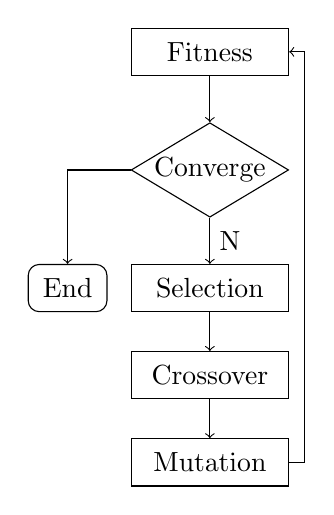
\begin{tikzpicture}
	\tikzstyle{startstop} = [rectangle, rounded corners, minimum width=1.0cm,minimum height=0.6cm, text centered, draw=black]
    \tikzstyle{io} = [trapezium, trapezium left angle=70, trapezium right angle=110, minimum width=2cm, minimum height=0.6cm, text centered, draw=black]
    \tikzstyle{process} = [rectangle, minimum width=2cm, minimum height=0.6cm, text centered, draw=black]
    \tikzstyle{decision} = [diamond,minimum width=2cm, minimum height=1.2cm, draw=black]
    \node (fitness) [process] {Fitness};
    \node[yshift=-0.5cm] (decision) [decision, below of=fitness] {} node at (decision.base) {Converge};
    \node[yshift=-0.5cm] (selection) [process, below of=decision] {Selection};
    \node (crossover) [process] at ($(selection.south)+(0,-0.8cm)$) {Crossover};
    \node (mutation) [process] at ($(crossover.south)+(0,-0.8cm)$)  {Mutation};
    \node (end) [startstop] at ($(selection.west)+(-0.8cm,0cm)$) {End};

    \draw [->] (fitness) -- (decision);
    \draw [->] (decision.south) -- (selection.north) node[auto=left,pos=0.5]{N};
    \draw [->] (selection.south) -- (crossover.north);
    \draw [->] (crossover.south) -- (mutation.north);
    \draw [->] (decision.west) -| (end.north);
	\draw [->] (mutation.east) -- ($(mutation.east)+(0.2cm,0cm)$) |-
		(fitness.east);
\end{tikzpicture}
\end{center}
\end{figure}
\end{document}
